\chapter{Rezultati}
\label{ch:rezultati}

V poglavju so rezultati predstavljeni glede na dokazno vrednost posameznega
preskusa. Najprej podajamo razvojni rezultat končnega sedemrazrednega modela
YAMNet-1024, nato rezervirani fizični preskus predhodne izvedbe YAMNet-256 in
nadzorovani sprejemni preskus med razvojem. Primarni rezultat predstavlja
neodvisni končni fizični preizkus s 60 posnetki. Rezultatov različnih stopenj
ne združujemo, saj so bile izvedene z različnimi modeli in nameni. Na koncu so
predstavljeni še izmerjeni časi izvajanja,
pomnilniški odtis in računska zahtevnost končne izvedbe.

\section{Razvojni rezultat končnega modela}
\label{sec:rezultati-razvojni}

Končni sedemrazredni model YAMNet-1024 je na razvojnem naboru pravilno
razvrstil 333 od 413 posnetkov, kar pomeni \SI{80.6}{\percent}. Posamezni
posnetki so bili razdeljeni na krajše obdelovalne izseke. Med 2.961 takšnimi
izseki jih je bilo pravilno razvrščenih 2.080 oziroma \SI{70.2}{\percent}.
Rezultat celotnega posnetka je boljši, ker se pri združevanju več zaporednih
izsekov zmanjša vpliv posamezne kratkotrajne napačne napovedi.

Makro povprečje natančnosti je znašalo 0,788, makro povprečje priklica 0,844,
makro mera $F_1$ pa 0,806. Natančnost pri tem pove, kolikšen delež napovedi
določenega razreda je bil pravilen, priklic pa, kolikšen delež dejanskih
primerov tega razreda je model našel. Makro povprečje vsakemu razredu pripiše
enako težo, ne glede na različno število posnetkov po razredih.

\begin{table}[!ht]
  \centering
  \caption{Rezultati končnega modela YAMNet-1024 na razvojnem naboru.}
  \label{tab:razvojni-rezultati-1024}
  \small
  \begin{tabular}{lrrrr}
    \toprule
    Razred & Pravilno & Natančnost & Priklic & Mera $F_1$ \\
    \midrule
    Pasji lajež       & 47 od 60  & 0,904 & 0,783 & 0,839 \\
    Razbitje stekla   & 41 od 60  & 0,854 & 0,683 & 0,759 \\
    Strel             & 48 od 54  & 0,828 & 0,889 & 0,857 \\
    Ostalo            & 98 od 135 & 0,810 & 0,726 & 0,766 \\
    Sirena            & 18 od 20  & 0,667 & 0,900 & 0,766 \\
    Govor             & 23 od 24  & 0,639 & 0,958 & 0,767 \\
    Nevihta           & 58 od 60  & 0,817 & 0,967 & 0,885 \\
    \midrule
    Makro povprečje   & --         & 0,788 & 0,844 & 0,806 \\
    \bottomrule
  \end{tabular}
\end{table}

Najvišjo mero $F_1$ je dosegla nevihta, sledila sta strel in pasji lajež.
Razred ostalo je pravilno zajel 98 od 135 razvojnih posnetkov. Njegov priklic
0,726 kaže, da je del raznolikih običajnih zvokov še vedno prešel v druge
razrede. Pri govoru je bil priklic visok, natančnost pa nižja, ker je model kot
govor označil tudi nekaj drugih človeških ali okoliških zvokov. Rezultati so
bili uporabljeni pri izbiri modela in nastavitvi pragov, zato niso neodvisna
končna ocena delovanja v poljubnem okolju.

\section{Rezervirani preskus predhodne izvedbe}
\label{sec:rezultati-rezervirani}

Rezervirani fizični preskus je ovrednotil predhodno izvedbo YAMNet-256. Med 60
pozitivnimi poskusi se je pričakovani razred pojavil kot potrjena odločitev v
37 primerih. Opaženi delež je bil zato \SI{61.7}{\percent}, njegovo
petindevetdesetodstotno Wilsonovo območje zaupanja pa od \SI{49.0}{\percent}
do \SI{72.9}{\percent}. Če govor izločimo in upoštevamo samo pet nevarnostnih
razredov, je bilo pravilnih 27 od 50 poskusov oziroma \SI{54.0}{\percent}.

\begin{table}[!ht]
  \centering
  \caption{Rezervirani fizični preskus predhodne izvedbe YAMNet-256.}
  \label{tab:rezervirani-rezultati-256}
  \small
  \begin{tabular}{lrrrr}
    \toprule
    Razred & Potrjeno & Prvo mesto & Delež & \shortstack{Wilsonovo območje\\zaupanja} \\
    \midrule
    Pasji lajež       & 6 od 10  & 9 od 10  & \SI{60}{\percent}  & 31,3--83,2 \\
    Razbitje stekla   & 5 od 10  & 9 od 10  & \SI{50}{\percent}  & 23,7--76,3 \\
    Strel             & 3 od 10  & 7 od 10  & \SI{30}{\percent}  & 10,8--60,3 \\
    Sirena            & 9 od 10  & 9 od 10  & \SI{90}{\percent}  & 59,6--98,2 \\
    Govor             & 10 od 10 & 9 od 10  & \SI{100}{\percent} & 72,2--100 \\
    Nevihta           & 4 od 10  & 8 od 10  & \SI{40}{\percent}  & 16,8--68,7 \\
    \midrule
    Skupaj            & 37 od 60 & --        & \SI{61.7}{\percent} & 49,0--72,9 \\
    \bottomrule
  \end{tabular}
\end{table}

Stolpec \emph{prvo mesto} v tabeli \ref{tab:rezervirani-rezultati-256} pove,
da je imel pričakovani razred v vsaj enem aktivnem bloku najvišjo glajeno
oceno. To še ne pomeni potrjene odločitve. Pri strelu je bil pričakovani razred
na prvem mestu v sedmih poskusih, potrjen pa le v treh. Podobna razlika je bila
vidna pri razbitju stekla in nevihti. Model je torej pogosto našel ustrezno
zvočno značilnost, vendar dokaz ni bil dovolj močan ali dovolj dolgotrajen, da
bi prestal pogoje odločitvenega filtra. To opažanje je bilo glavni razlog za
poznejšo izboljšavo izrezovanja kratkotrajnih dogodkov, povečanje učnih podatkov
in prehod na večji model.

\begin{figure}[!ht]
  \centering
  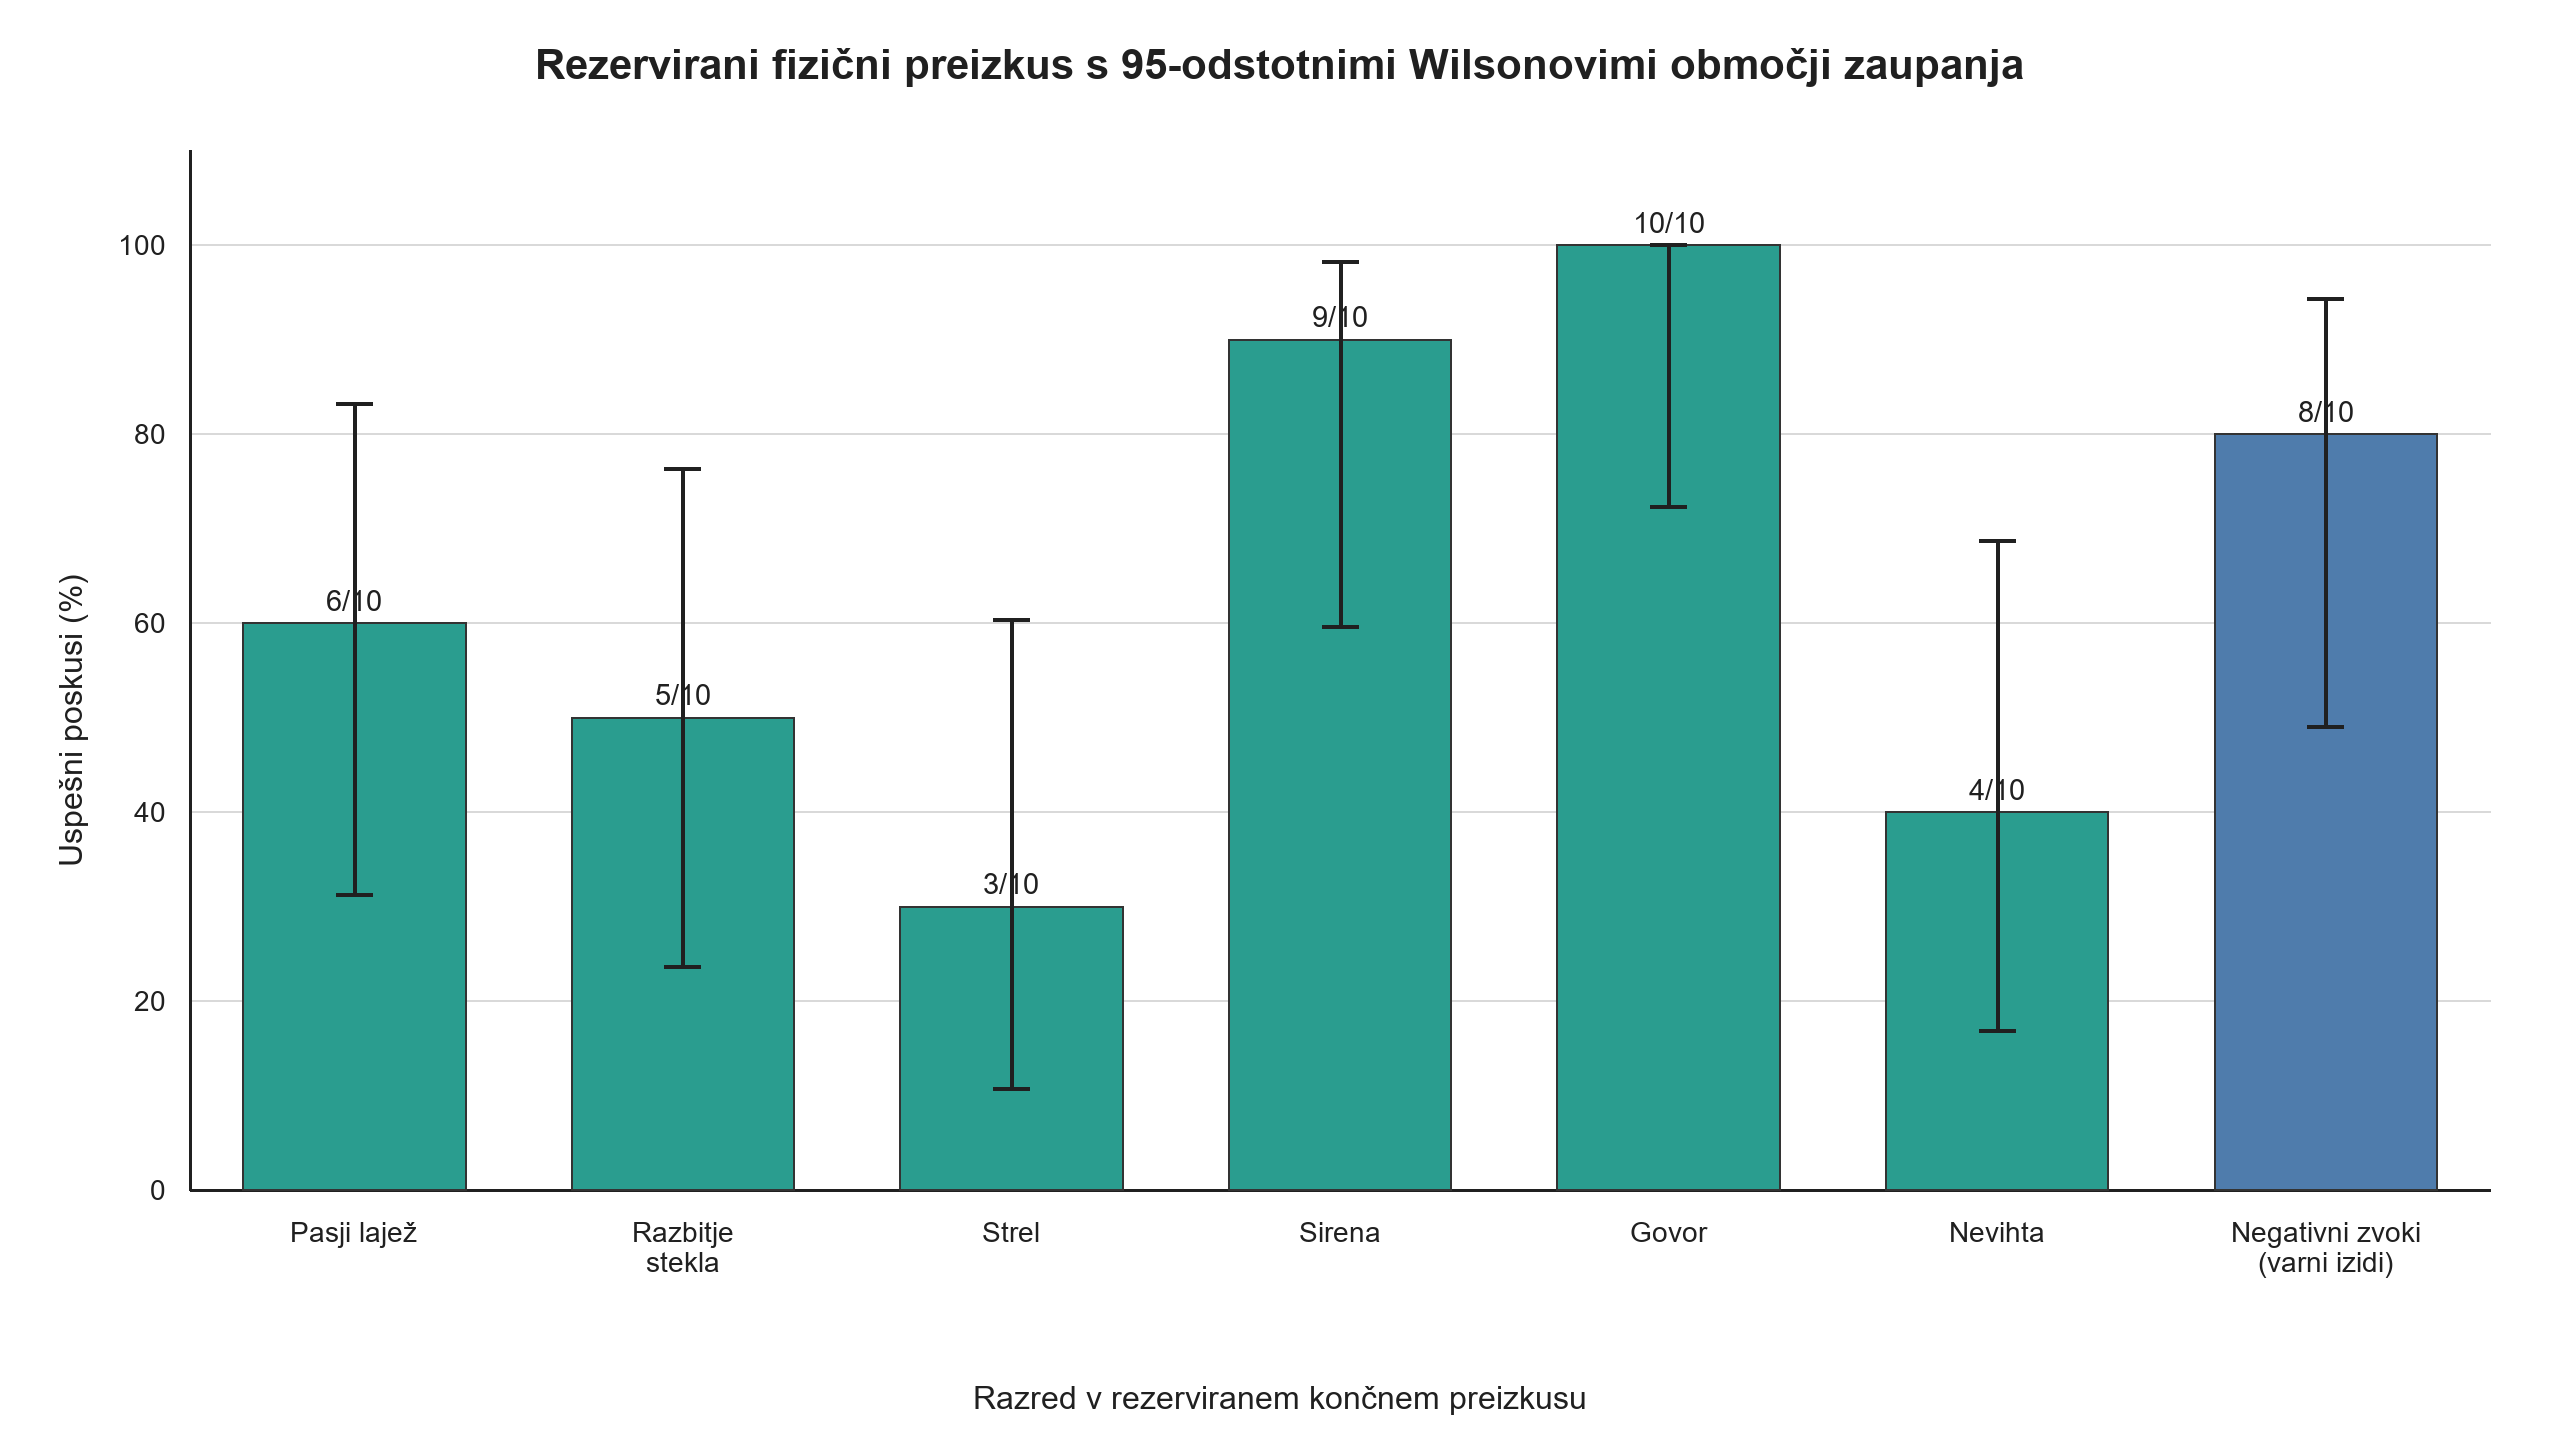
\includegraphics[width=0.94\textwidth]{../experiments/results/thesis_ch6/reserved_detection_rates_sl.png}
  \caption{Potrjene zaznave predhodne izvedbe YAMNet-256. Črte prikazujejo
  petindevetdesetodstotna Wilsonova območja zaupanja. Pri zahtevnih negativnih
  zvokih je prikazan delež varnih izidov.}
  \label{fig:rezervirani-delezi}
\end{figure}
\clearpage

\section{Lažni alarmi predhodne izvedbe}

Govor je bil v model vključen kot varen razred, da običajnega človeškega glasu
ne bi zamenjeval z nevarnostjo. Kljub pravilno zaznanemu govoru v vseh desetih
pozitivnih poskusih je v enem od njih za kratek čas nastal tudi potrjen
nevarnostni izhod. Opaženi delež takšnih lažnih alarmov je bil zato 1 od 10.

Med desetimi zahtevnimi negativnimi zvoki sta dva sprožila potrjen nevarnostni
alarm, osem pa jih je imelo varen izid. Šest od desetih primerov ni preseglo
praga vhodne aktivnosti. To ni napaka prenosa zvoka, temveč odziv naprave pri
izbranem pragu: obdelava je zvok prejela, vendar ga ni obravnavala kot dovolj
izrazitega za odločanje. Zaradi samo desetih negativnih primerov rezultat
\SI{20}{\percent} lažnih nevarnostnih alarmov opisuje ta preskus in ni ocena
pričakovane pogostosti lažnih alarmov pri dolgotrajni uporabi.

\section{Sprejemni preskus končne naprave}
\label{sec:rezultati-sprejemni}

Končna naprava z modelom YAMNet-1024 je uspešno opravila 18 od 21 poskusov
nadzorovanega sprejemnega preskusa, kar pomeni \SI{85.7}{\percent}. Pri
nominalni ravni je bilo uspešnih 8 od 9 poskusov oziroma
\SI{88.9}{\percent}. Med 18 pozitivnimi poskusi je bil pričakovani razred
potrjen v 15 primerih, vsi trije varni negativni zvoki pa so bili obravnavani
brez potrjenega nevarnostnega alarma.

\begin{table}[H]
  \centering
  \caption{Uspešnost sprejemnega preskusa končne naprave po razredih.}
  \label{tab:sprejemni-rezultati-razredi}
  \begin{tabular}{lrrrr}
    \toprule
    Razred & Nominalno & \SI{-6}{\decibel} & \SI{-12}{\decibel} & Skupaj \\
    \midrule
    Pasji lajež       & 1 od 1 & 1 od 1 & 1 od 1 & 3 od 3 \\
    Razbitje stekla   & 1 od 1 & 1 od 1 & 0 od 1 & 2 od 3 \\
    Strel             & 1 od 1 & 1 od 1 & 1 od 1 & 3 od 3 \\
    Sirena            & 1 od 1 & 1 od 1 & 1 od 1 & 3 od 3 \\
    Govor             & 1 od 1 & 1 od 1 & 0 od 1 & 2 od 3 \\
    Nevihta           & 0 od 1 & 1 od 1 & 1 od 1 & 2 od 3 \\
    \midrule
    Pozitivni zvoki   & 5 od 6 & 6 od 6 & 4 od 6 & 15 od 18 \\
    Varni zvoki       & 3 od 3 & --     & --     & 3 od 3 \\
    \bottomrule
  \end{tabular}
\end{table}

Pasji lajež, strel in sirena so bili uspešno potrjeni pri vseh treh ravneh.
Razbitje stekla in govor pri ravni \SI{-12}{\decibel} nista presegla praga
vhodne aktivnosti. Pri nevihti na nominalni ravni je bil pričakovani razred v
več aktivnih blokih na prvem mestu, vendar ni bil v dveh zaporednih blokih
dovolj močan za potrditev. To je edini neuspeh, pri katerem je dogodek prestal
energijski prag, ustavil pa ga je odločitveni pogoj.

\begin{figure}[!ht]
  \centering
  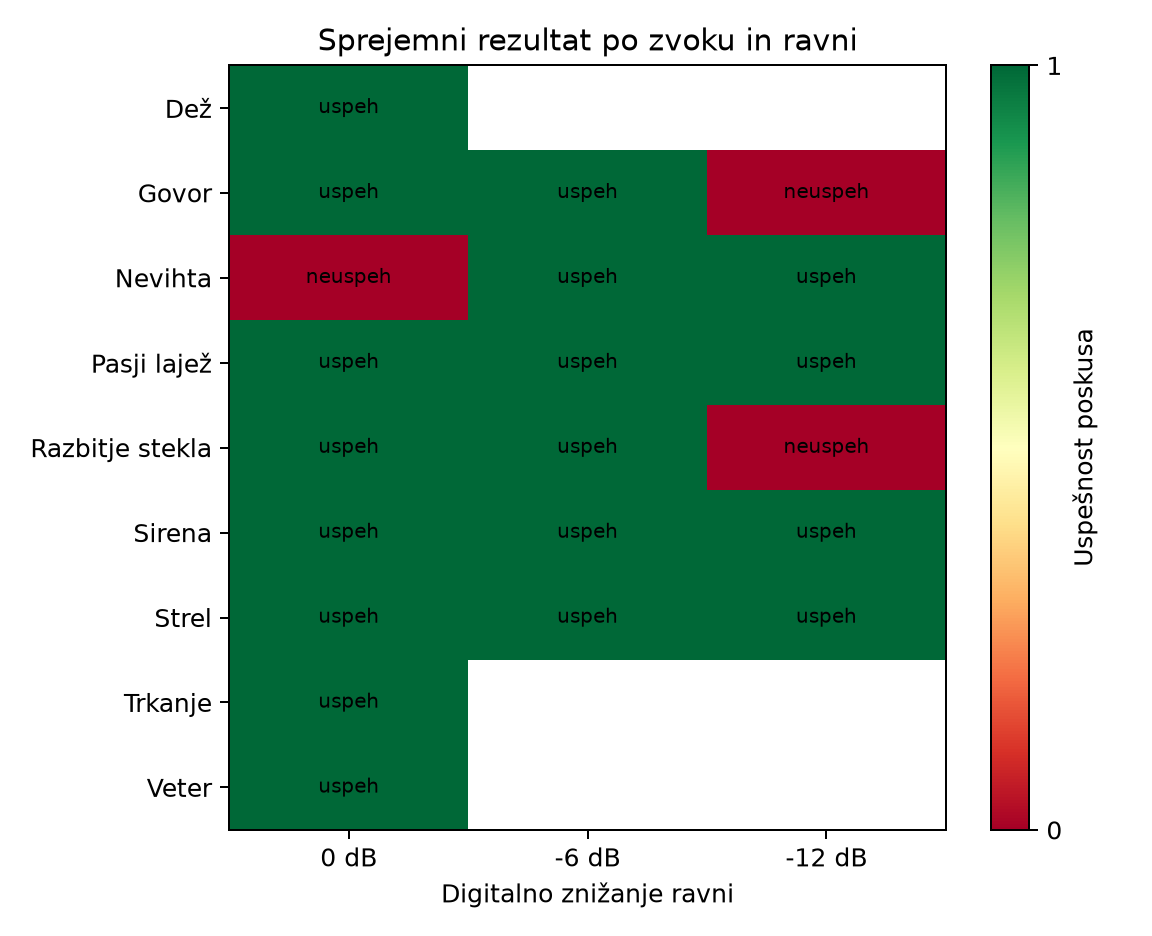
\includegraphics[width=0.94\textwidth]{../experiments/results/hazard6_v3_acceptance/trial_matrix.png}
\caption{Izid posameznih poskusov sprejemnega preskusa končne naprave.}
  \label{fig:sprejemni-matrika}
\end{figure}

\begin{figure}[!ht]
  \centering
  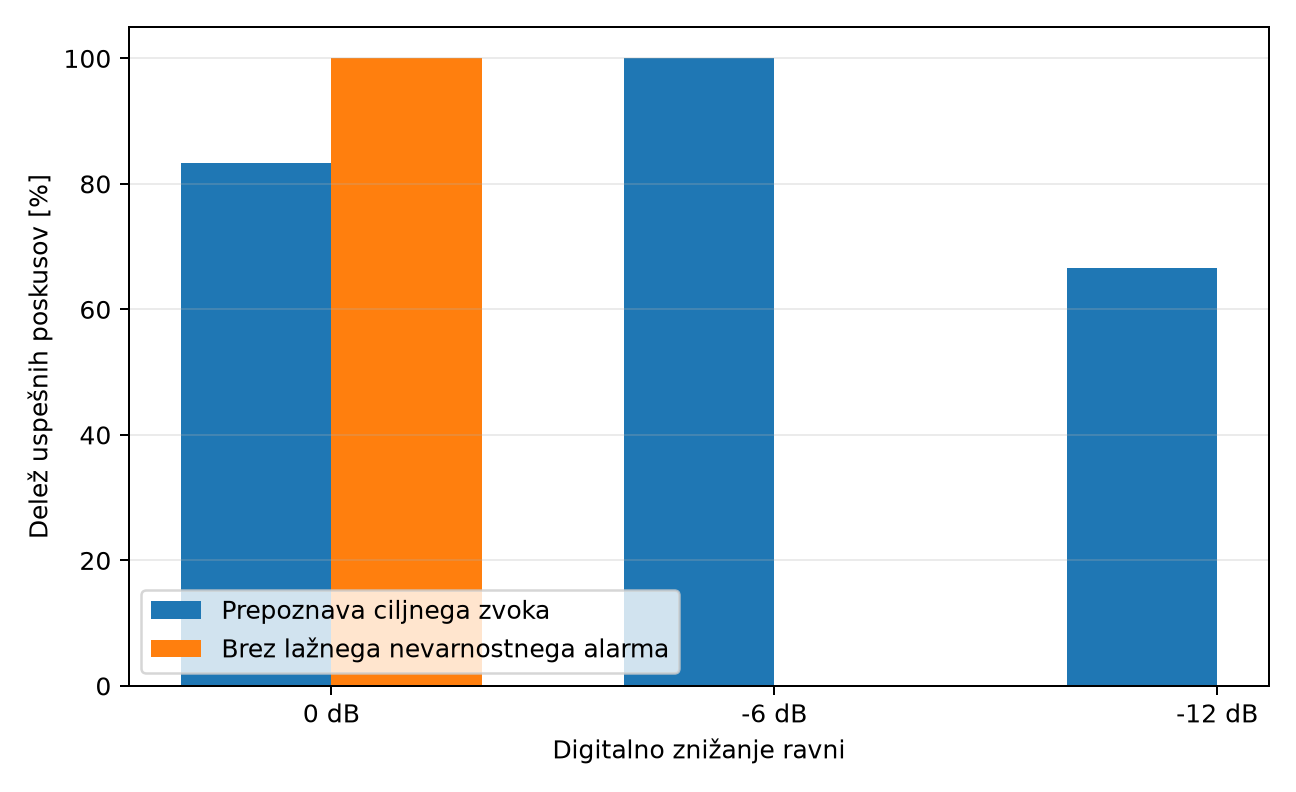
\includegraphics[width=0.82\textwidth]{../experiments/results/hazard6_v3_acceptance/pass_rate_by_level.png}
  \caption{Opaženi delež uspešnih poskusov pri posamezni ravni predvajanja.}
  \label{fig:sprejemni-ravni}
\end{figure}
\clearpage

Pri pozitivnih poskusih je bil delež uspeha pri nominalni ravni
\SI{83.3}{\percent}, pri \SI{-6}{\decibel} \SI{100}{\percent} in pri
\SI{-12}{\decibel} \SI{66.7}{\percent}. Iz tega ne smemo sklepati, da
utišanje izboljša zaznavanje. Vsaka kombinacija posnetka in ravni je bila
predvajana samo enkrat, rezultat kratkega dogodka pa je odvisen tudi od njegove
poravnave z mejo obdelovalnega bloka ter trenutnega šuma v prostoru. Preskus zato
predvsem potrjuje, da celotna končna izvedba deluje na izbranih in predhodno
pregledanih primerih. Ne predstavlja neodvisne ocene posploševanja modela na
nove zvočne vire.

\section{Neodvisni končni fizični preizkus}
\label{sec:rezultati-koncni}

V neodvisnem končnem fizičnem preizkusu je sistem pričakovani razred vsaj
enkrat potrdil v 57 od 60 poskusov. Opaženi delež je
\SI{95.0}{\percent}, Wilsonovo petindevetdesetodstotno območje zaupanja pa od
\SI{86.3}{\percent} do \SI{98.3}{\percent}. Štirje nevarnostni razredi skupaj
so bili potrjeni v 39 od 40 poskusov oziroma \SI{97.5}{\percent}.

\begin{table}[htbp]
  \centering
  \caption{Rezultati neodvisnega končnega fizičnega preizkusa.}
  \label{tab:koncni-rezultati}
  \small
  \begin{tabular}{lrrr}
    \toprule
    Razred & Uspešni poskusi & Delež & \shortstack{Wilsonovo območje\\zaupanja} \\
    \midrule
    Pasji lajež       & 10 od 10 & \SI{100}{\percent} & 72,2--100 \\
    Razbitje stekla   & 10 od 10 & \SI{100}{\percent} & 72,2--100 \\
    Strel             & 10 od 10 & \SI{100}{\percent} & 72,2--100 \\
    Ostalo            & 9 od 10  & \SI{90}{\percent}  & 59,6--98,2 \\
    Sirena            & 9 od 10  & \SI{90}{\percent}  & 59,6--98,2 \\
    Govor             & 9 od 10  & \SI{90}{\percent}  & 59,6--98,2 \\
    \midrule
    Skupaj            & 57 od 60 & \SI{95.0}{\percent} & 86,3--98,3 \\
    \bottomrule
  \end{tabular}
\end{table}

\begin{figure}[htbp]
  \centering
  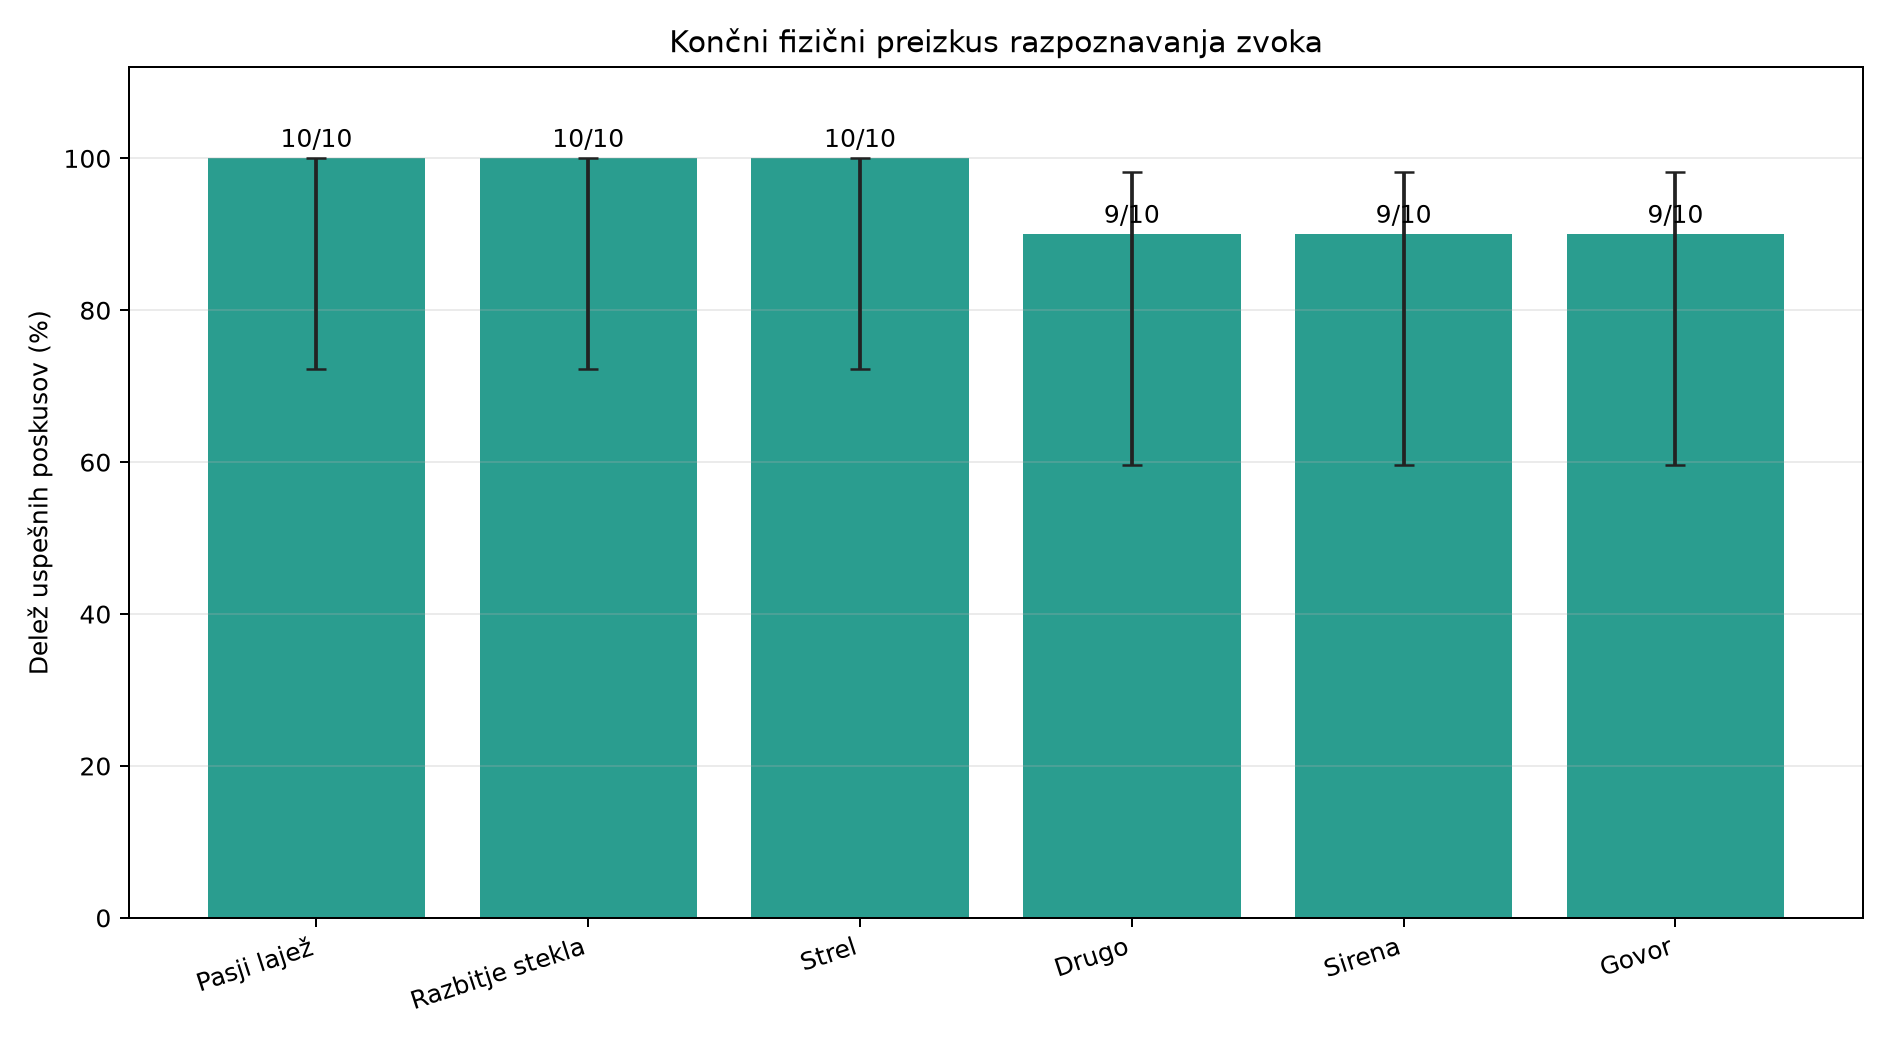
\includegraphics[width=0.96\textwidth]{../experiments/results/hazard6_final_evaluation_v4_independent/detection_rates.png}
  \caption{Delež poskusov z vsaj eno pravilno potrditvijo v neodvisnem
  končnem preizkusu. Črte prikazujejo Wilsonova petindevetdesetodstotna
  območja zaupanja.}
  \label{fig:koncni-delezi}
\end{figure}

Primarno merilo poskus šteje kot uspešen že ob eni pravilni potrditvi. Strožje
merilo prevladujočega potrjenega izhoda se je s pričakovanim razredom ujemalo v
54 od 60 poskusov oziroma \SI{90.0}{\percent}. Razlika nastane, kadar sistem
pričakovani razred sicer potrdi, vendar je drug izhod med istim predvajanjem
potrjen v več blokih. En poskus strela je imel tako prevladujoči izhod
razbitja stekla, dva uspešna govorna poskusa pa prevladujoči izhod ostalo.

\begin{figure}[htbp]
  \centering
  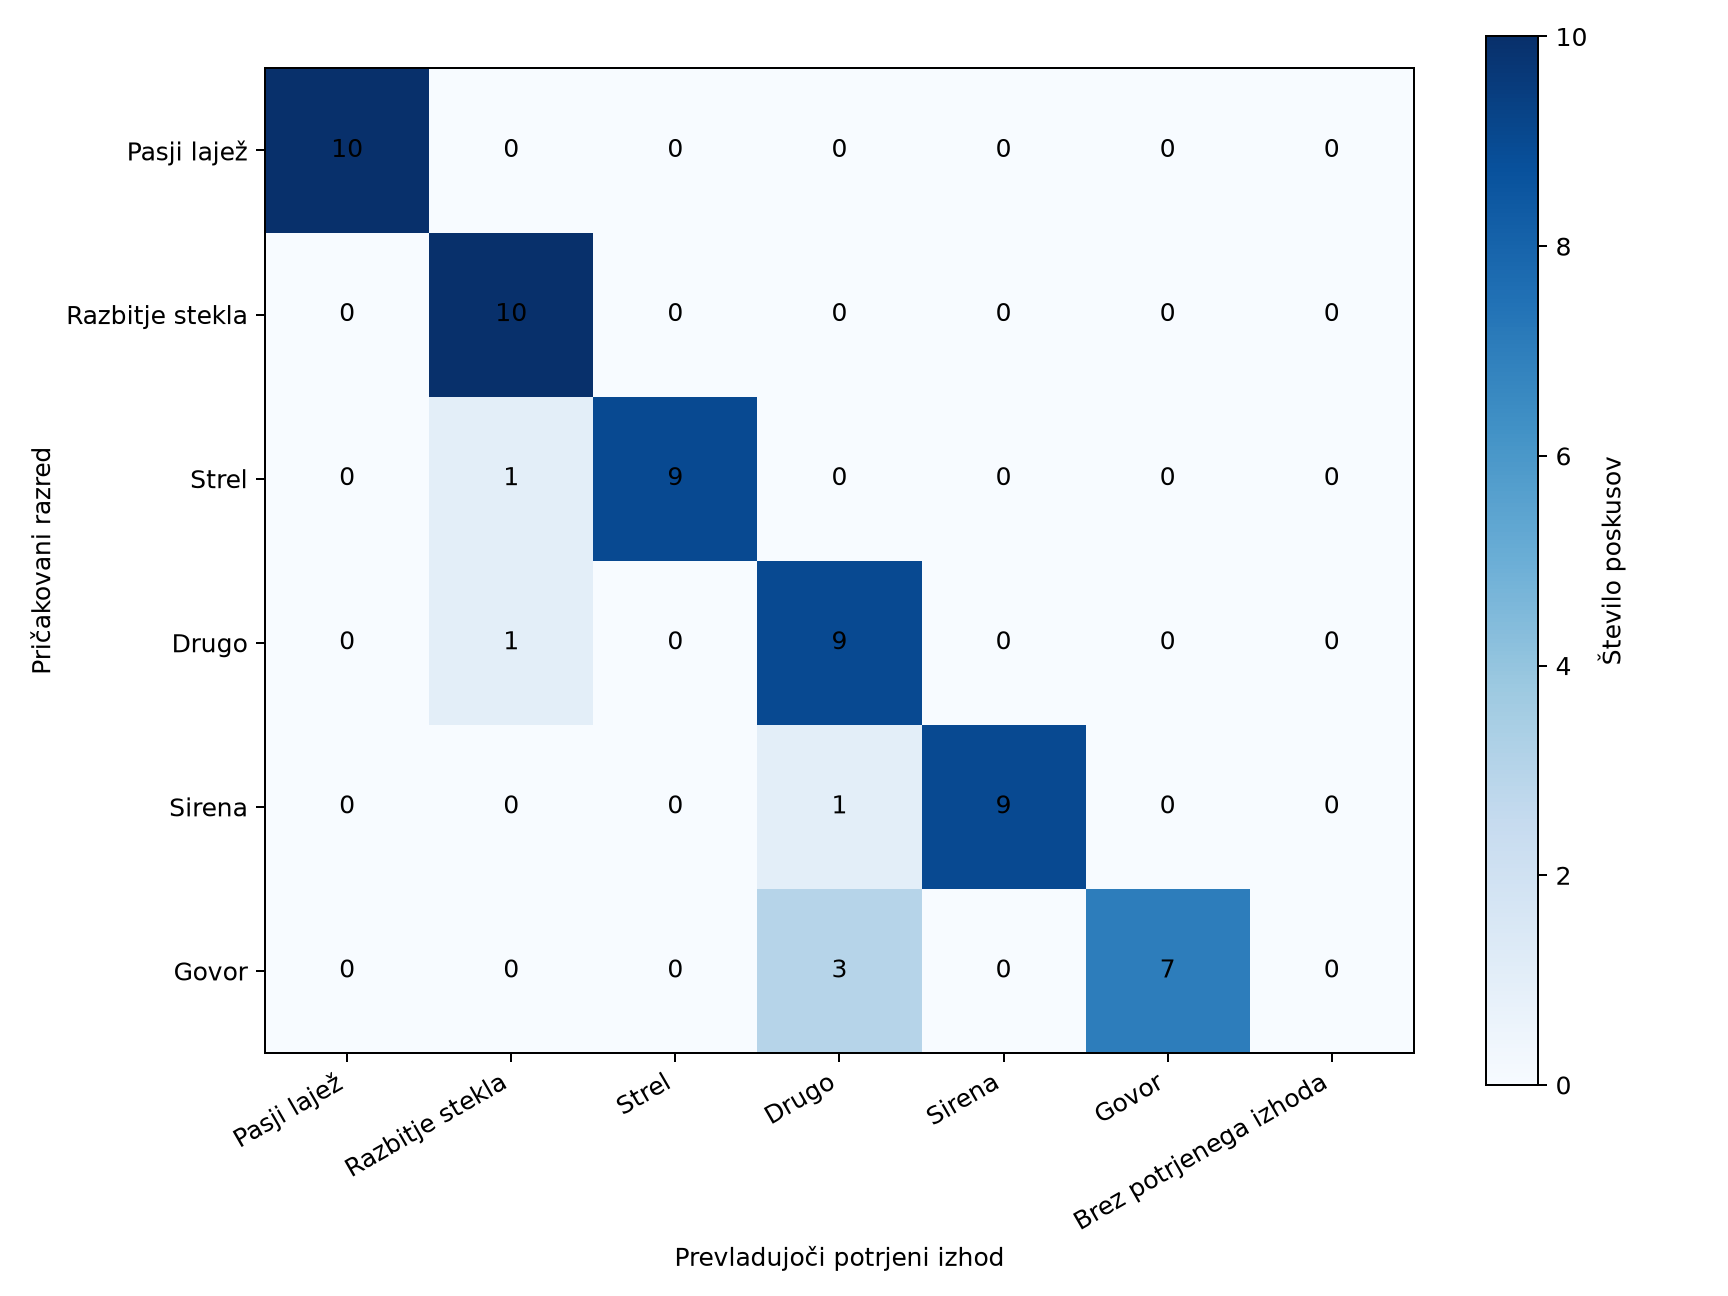
\includegraphics[width=0.88\textwidth]{../experiments/results/hazard6_final_evaluation_v4_independent/dominant_output_confusion_matrix.png}
  \caption{Matrika prevladujočih potrjenih izhodov. Primarno merilo na sliki
  \ref{fig:koncni-delezi} je drugačno, ker upošteva vsaj eno pravilno
  potrditev.}
  \label{fig:koncni-matrika}
\end{figure}

Trije neuspešni poskusi so zbrani v tabeli \ref{tab:koncni-neuspehi}. Pri
govoru je najvišja ocena pričakovanega razreda znašala 0,357 in ni dosegla
vstopnega praga 0,40. Kratek pok razreda ostalo je bil v 17 blokih potrjen
kot razbitje stekla. Pri neuspešni sireni je modelska ocena sirene dosegla
0,595, kar je ostalo pod pragom 0,65; prevladujoči potrjeni izhod je bil ostalo.

\begin{table}[htbp]
  \centering
  \caption{Neuspešni poskusi neodvisnega končnega preizkusa.}
  \label{tab:koncni-neuspehi}
  \small
  \begin{tabular}{llllr}
    \toprule
    Poskus & Pričakovano & Vrsta vira & Prevladujoči izhod & Najvišja ocena \\
    \midrule
    FE4-010 & Govor  & govor  & Ostalo            & 0,357 \\
    FE4-032 & Ostalo & pok    & Razbitje stekla   & 0,360 \\
    FE4-058 & Sirena & sirena & Ostalo            & 0,595 \\
    \bottomrule
  \end{tabular}
\end{table}

\subsection{Lažni nevarnostni alarmi}

Pri desetih govornih poskusih po začetku predvajanja ni bilo nobenega
potrjenega nevarnostnega izhoda. Pri razredu ostalo se je nevarnostni izhod vsaj
enkrat pojavil v šestih od desetih poskusov. V štirih od skupno 20 varovalnih
poskusov je ostal potrjen v več kot enem bloku. En dodaten nevarnostni izhod je bil v
celotnem zajemu govora zabeležen pred začetkom predvajanja; analiza ga je
pravilno ločila kot preneseno stanje prejšnjega poskusa.

Rezultat 9 od 10 pravilnih zaznav razreda ostalo in šest poskusov z lažnim
alarmom se ne izključujeta. V petih poskusih je sistem v delu predvajanja
pravilno potrdil ostalo, v drugem delu istega posnetka pa tudi nevarnostni
razred. Slika \ref{fig:koncni-lazni-ostalo} pokaže, da je bil najtežji pok, ki
je prevladal kot razbitje stekla. Pri aplavzu je bil strel potrjen v štirih
blokih, ploskanje, tipkovnica, alarm in trkanje pa so povzročili krajše
potrditve razbitja stekla.

\begin{figure}[htbp]
  \centering
  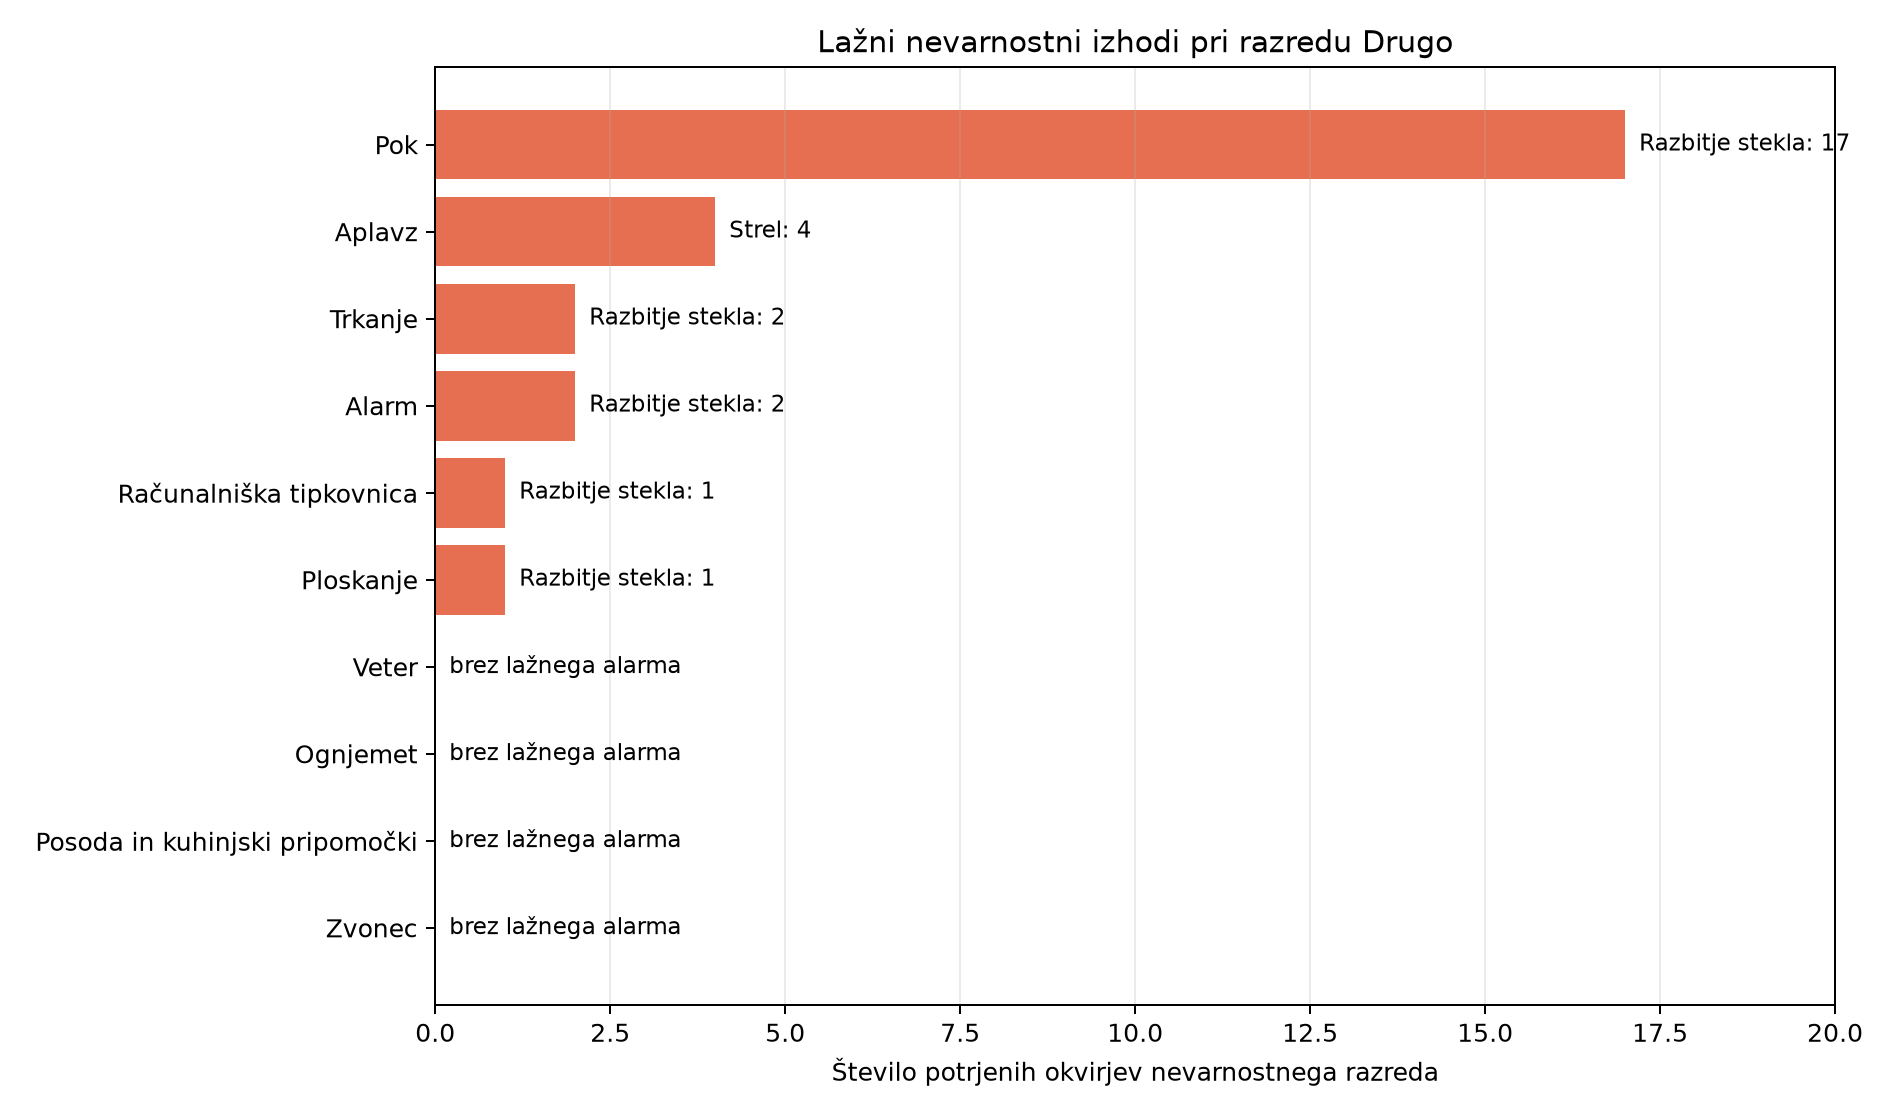
\includegraphics[width=0.96\textwidth]{../experiments/results/hazard6_final_evaluation_v4_independent/other_false_hazard_by_category.png}
  \caption{Število blokov s potrjenim nevarnostnim izhodom pri desetih vrstah
  razreda ostalo.}
  \label{fig:koncni-lazni-ostalo}
\end{figure}

\subsection{Čas do prve pravilne potrditve}

Mediana časa od začetka predvajanja do prve pravilne potrditve je bila med
\SI{1.00}{\second} za razbitje stekla in \SI{2.50}{\second} za razred ostalo.
Pri tem ne merimo samo računanja modela. Vrednost vključuje morebitno tišino
na začetku posnetka, položaj dogodka, zbiranje skoraj enosekundnega vhodnega
bloka in zahtevano število potrditvenih blokov.

\begin{figure}[htbp]
  \centering
  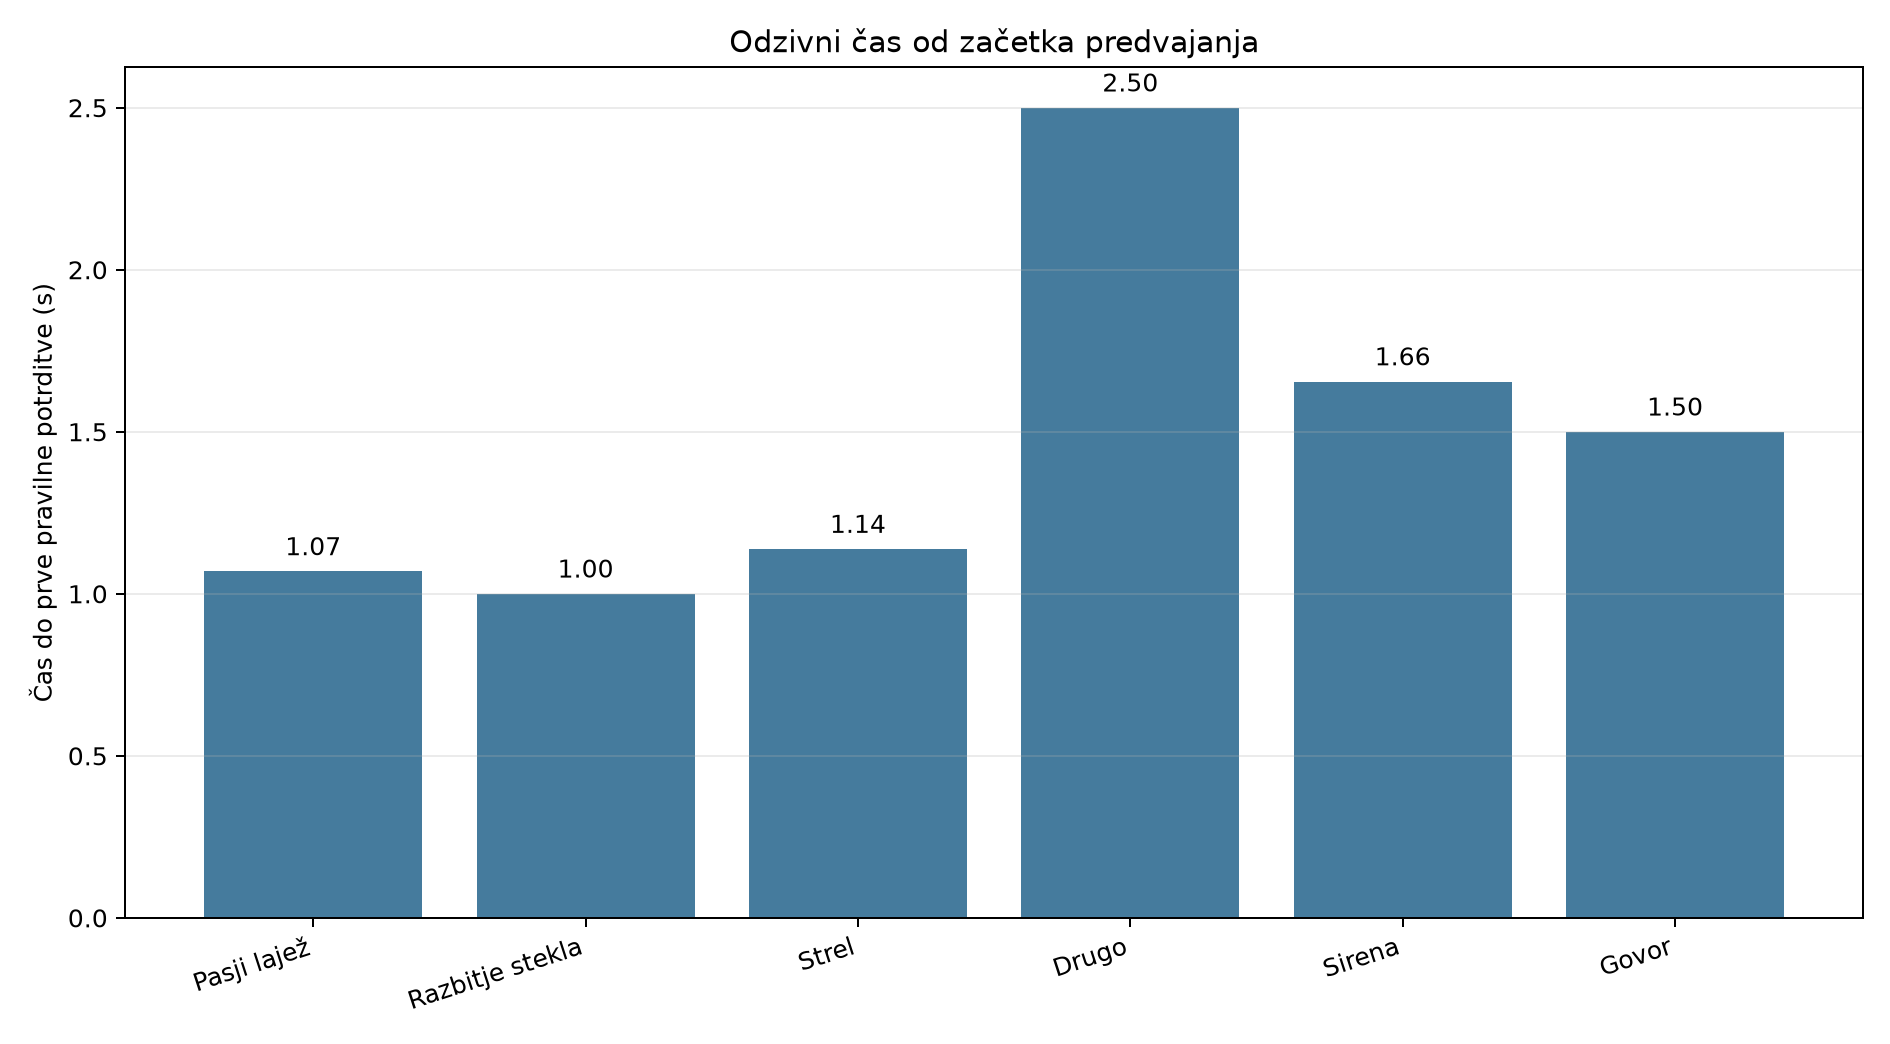
\includegraphics[width=0.94\textwidth]{../experiments/results/hazard6_final_evaluation_v4_independent/confirmation_latency.png}
  \caption{Mediana časa od začetka predvajanja do prve pravilne potrditve.}
  \label{fig:koncni-odzivni-cas}
\end{figure}

\section{Čas izvajanja}
\label{sec:rezultati-cas}

V rezerviranem preskusu izvedbe YAMNet-256 je bilo zbranih 1.438 časovnih
opazovanj. Pri sprejemnem preskusu prve šestrazredne izvedbe YAMNet-1024 je
bilo 269 popolnih zapisov, neodvisni končni preizkus sedemizhodne izvedbe pa je
vseboval 1.837 popolnih časovnih zapisov. Povprečni in mediani so bili v
zadnjem preskusu enaki zaradi ločljivosti poročane telemetrije. Časi so zbrani
v tabeli \ref{tab:primerjava-casov}.

\begin{table}[H]
  \centering
  \caption{Čas obdelave enega vhodnega bloka na napravi.}
  \label{tab:primerjava-casov}
  \small
  \begin{tabular}{lrrr}
    \toprule
    Stopnja & YAMNet-256 & \shortstack{Prvi\\YAMNet-1024} & \shortstack{Končni\\YAMNet-1024} \\
    \midrule
    Predobdelava & \SI{0.69}{\milli\second} & \SI{0.71}{\milli\second} & \SI{1.43}{\milli\second} \\
    Izvajanje nevronske mreže & \SI{0.16}{\milli\second} & \SI{4.63}{\milli\second} & \SI{9.38}{\milli\second} \\
    Skupaj & \SI{0.85}{\milli\second} & \SI{5.34}{\milli\second} & \SI{10.81}{\milli\second} \\
    \bottomrule
  \end{tabular}
\end{table}

\begin{figure}[H]
  \centering
  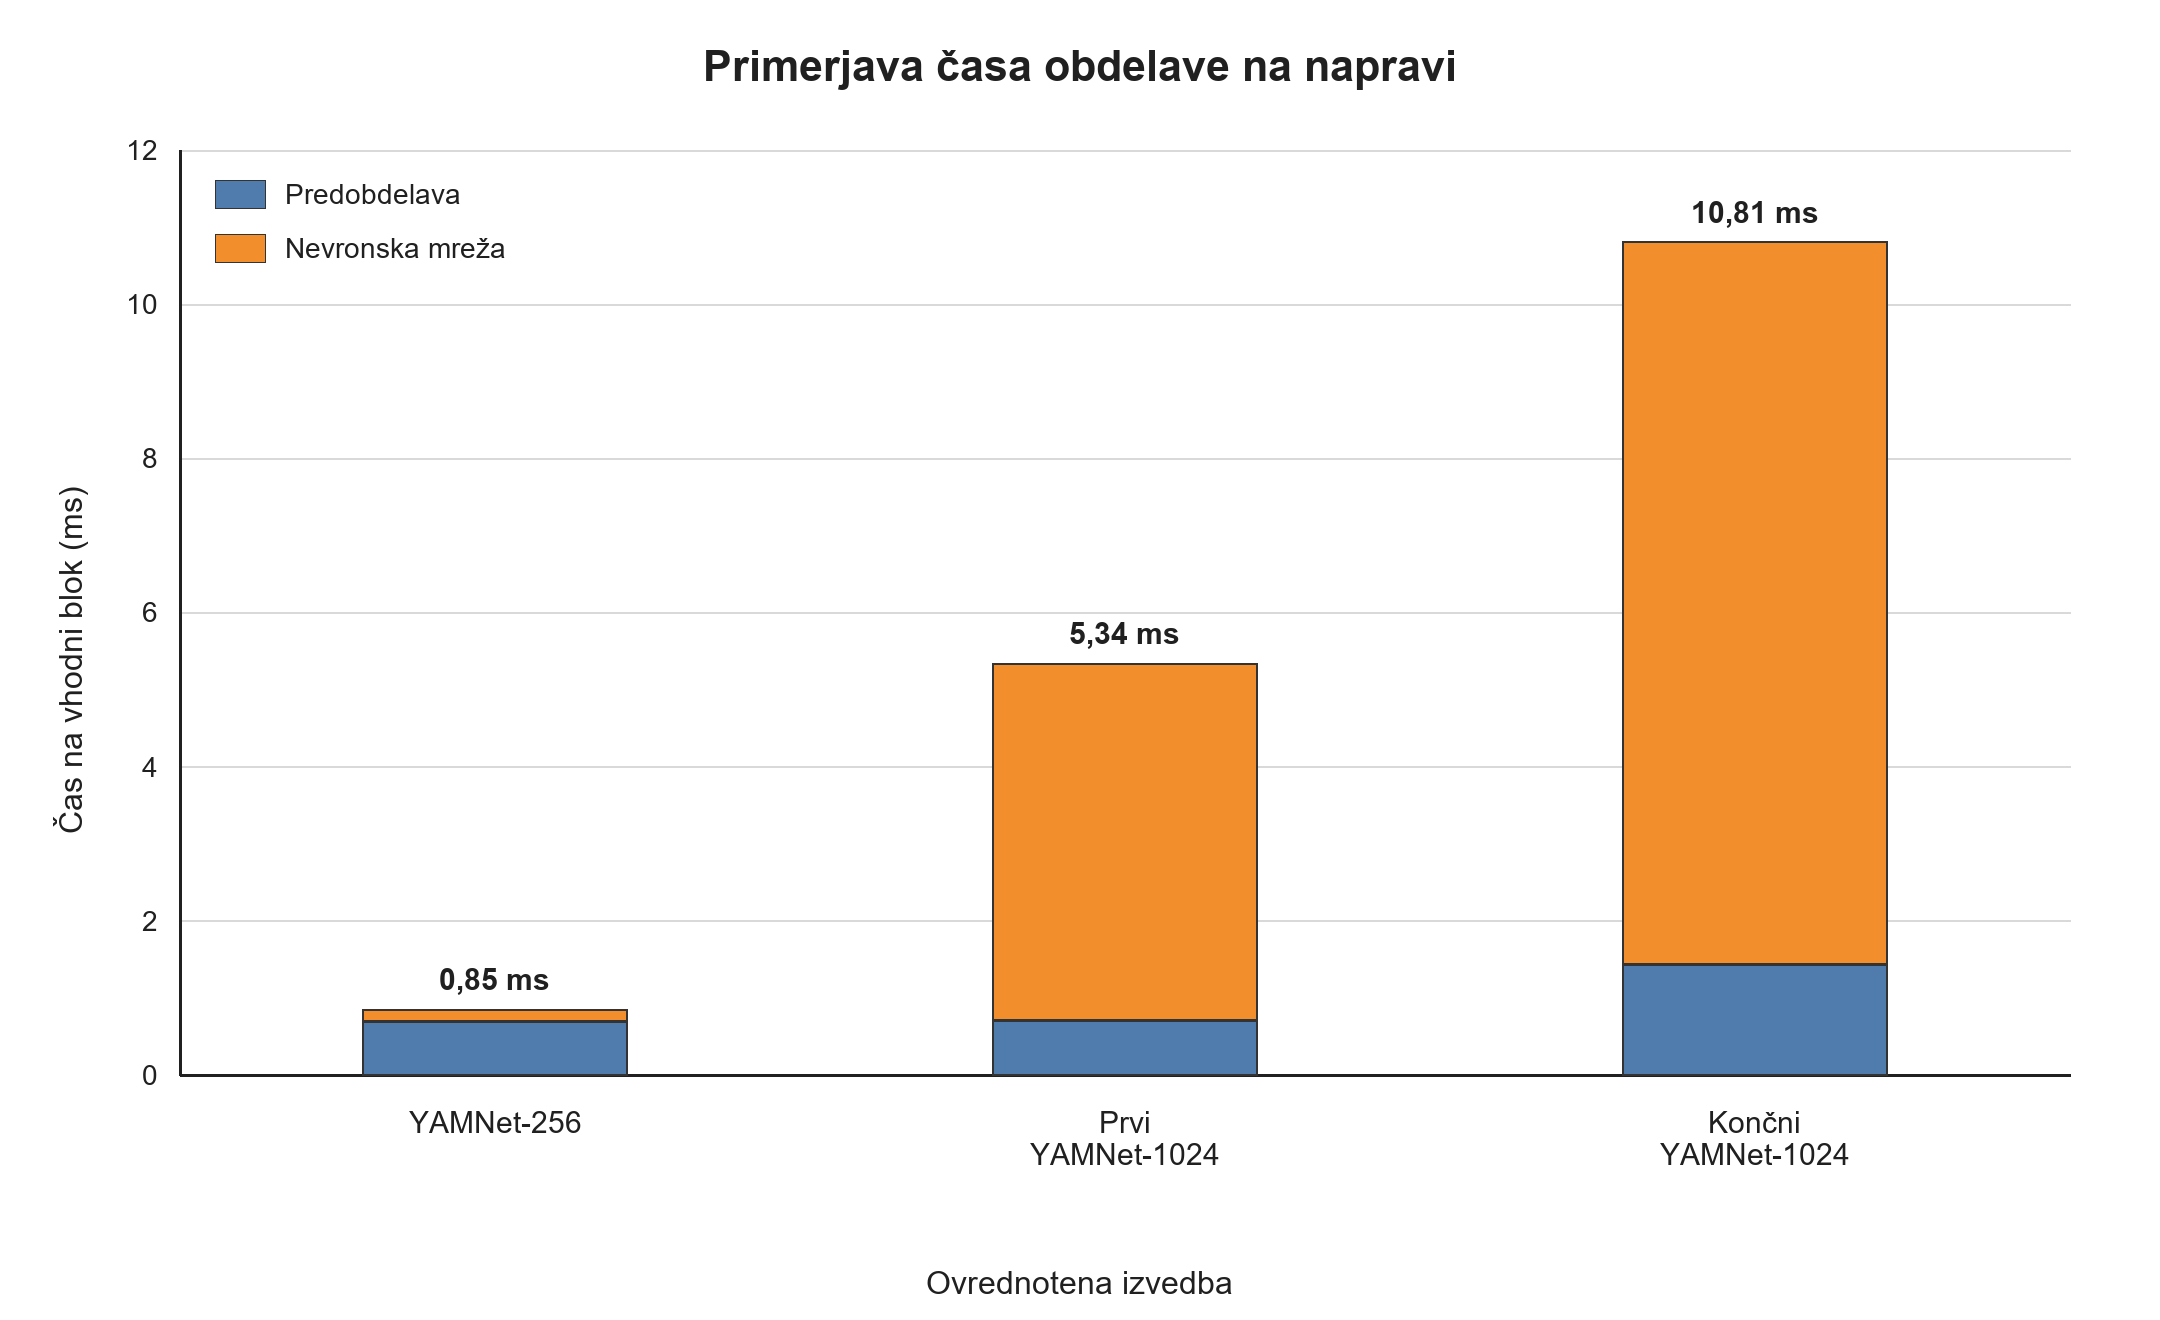
\includegraphics[width=0.88\textwidth]{../experiments/results/thesis_ch6/timing_comparison_sl.png}
  \caption{Primerjava časov obdelovalnih stopenj treh ovrednotenih izvedb.}
  \label{fig:primerjava-casov}
\end{figure}

Končna različica je zaradi večjega modela YAMNet in dodatnega izhoda
računsko zahtevnejša od začetne. Kljub temu je skupnih
\SI{10.81}{\milli\second} približno 44-krat manj od
\SI{480}{\milli\second} med začetkoma dveh zaporednih obdelav. Računska pot
zasede približno \SI{2.25}{\percent} tega intervala, zato ostane dovolj rezerve
za zajem zvoka in osveževanje zaslona.

Izvedba istega modela samo na procesorskem jedru ni bila izmerjena, zato iz teh
rezultatov ne izpeljujemo številčnega faktorja pohitritve Neural-ART. Meritev
\SI{9.38}{\milli\second} opisuje prevedeno izvedbo, v kateri je 29 od 34
izvedbenih odsekov dodeljenih pospeševalniku.

Izmerjenih \SI{10.81}{\milli\second} ni celotna zakasnitev zaznave. Naprava mora
najprej zbrati vhodni zvočni blok, odločitveni filter pa lahko zahteva še
potrditev v naslednjem bloku. Meritev zato dokazuje veliko časovno rezervo
računske poti, ne pa odziva v nekaj milisekundah od nastanka zvoka.

\section{Pomnilniški in računski odtis}
\label{sec:rezultati-pomnilnik}

Tabela \ref{tab:pomnilniski-odtis} primerja pomnilniški odtis predhodne in
končne izvedbe. Vrednosti pripadajo različnim fizičnim pomnilniškim območjem,
zato jih med seboj ne seštevamo. Stolpec izrabe prikazuje zasedenost
razpoložljivega območja pri končni izvedbi.

\begin{table}[H]
  \centering
  \caption{Primerjava pomnilniškega odtisa izvedb YAMNet-256 in YAMNet-1024.}
  \label{tab:pomnilniski-odtis}
  \small
  \begin{tabular}{>{\raggedright\arraybackslash}p{0.30\textwidth}
                  >{\centering\arraybackslash}p{0.14\textwidth}
                  >{\centering\arraybackslash}p{0.14\textwidth}
                  >{\centering\arraybackslash}p{0.14\textwidth}
                  >{\centering\arraybackslash}p{0.10\textwidth}}
    \toprule
    Pomnilniško območje & YAMNet-256 & YAMNet-1024 & \shortstack{Na\\voljo} & Izraba \\
    \midrule
    Notranji pomnilnik aplikacije
      & 582,2 KiB & 595,1 KiB & 1.023 KiB & \SI{58.2}{\percent} \\
    Aktivacije nevronskega pospeševalnika
      & 144,0 KiB & 240,0 KiB & 448 KiB & \SI{53.6}{\percent} \\
    Zaslonska medpomnilnika v zunanjem pomnilniku
      & 1.500,0 KiB & 1.500,0 KiB & 16.384 KiB & \SI{9.2}{\percent} \\
    Podpisana programska slika
      & 229,9 KiB & 244,3 KiB & 512 KiB & \SI{47.7}{\percent} \\
    Prevedene uteži v zunanjem bliskovnem pomnilniku
      & 145,2 KiB & 3.203,7 KiB & 64.512 KiB & \SI{5.0}{\percent} \\
    \bottomrule
  \end{tabular}
\end{table}

Največja sprememba je nastala pri utežeh, ki so se povečale približno
22-krat, in pri aktivacijskem pomnilniku, ki se je povečal za približno
1,67-krat. Velikost povezane aplikacije v notranjem pomnilniku se je povečala
le za približno \SI{0.7}{\percent}, podpisana programska slika pa za približno
\SI{2.5}{\percent}. Zaslonska medpomnilnika sta ostala nespremenjena. Večji
model se zato ni približal omejitvi zunanjega bliskovnega pomnilnika, prav tako
pa je v območju za aktivacije ostalo približno \SI{46}{\percent} prostora.

Datoteka izvedljive in povezovalne oblike vsebuje tudi simbole in druge podatke
za razhroščevanje, zato njena velikost ni enaka velikosti programske slike na
napravi. Dejanska podpisana binarna slika končne aplikacije ima 250.176 bajtov,
povezovalnik pa za izvajanje aplikacije navaja 609.372 bajtov notranjega
pomnilnika.

Poročilo prevajalnika modela za en prehod navaja 71.146.316 operacij množenja
in seštevanja. Izvajalni načrt je razdeljen na 34 odsekov: 29 jih izvede
nevronski pospeševalnik, pet pa procesorsko jedro. Programsko izvedeni odseki
so povezani predvsem s pretvorbami na mejah modela in z njegovo zaključno
plastjo. Izraz \emph{odsek} tu ne pomeni učnega prehoda, temveč del že
naučenega omrežja, ki ga je prevajalnik dodelil določeni strojni enoti. Večino
računsko zahtevnih plasti tako izvede Neural-ART, kar omogoča izmerjeni čas
\SI{9.38}{\milli\second} kljub več kot 71 milijonom operacij.

\section{Povzetek rezultatov}

Rezultati kažejo potek od odkritih pomanjkljivosti do izboljšane končne
izvedbe. Rezervirani fizični preskus YAMNet-256 je dosegel 37 potrjenih pravilnih
zaznav v 60 pozitivnih poskusih in je pokazal predvsem šibkost pri strelu,
razbitju stekla in nevihti. Na podlagi teh ugotovitev so bili izboljšani izbor
dogodkov, povečanje učnih podatkov, prehod na YAMNet-1024 in odločitveno pravilo
za nevihto.

Končni razvojni model YAMNet-1024 je pravilno razvrstil 333 od 413 razvojnih
posnetkov. Neodvisni končni fizični preizkus je nato dosegel vsaj eno pravilno
potrditev v 57 od 60 poskusov, strožje merilo prevladujočega izhoda pa v 54 od
60 poskusov. Pri štirih nevarnostnih razredih je bilo pravilnih 39 od 40
poskusov. Glavna preostala pomanjkljivost je zavračanje nekaterih drugih
kratkih in izrazitih zvokov: nevarnostni izhod se je pojavil pri šestih od
desetih poskusov razreda ostalo, pri štirih pa je ostal potrjen v več kot enem
bloku.

Prehod na večji model in razširjeni razred ostalo sta povečala čas izvajanja in
pomnilniški odtis, vendar je končna izvedba ostala znotraj vseh pomnilniških
območij. Skupna obdelava enega bloka traja \SI{10.81}{\milli\second}, zato ima
sistem pri novem bloku vsakih \SI{480}{\milli\second} veliko časovno rezervo.
Rezultati potrjujejo delovanje celotne poti na izbrani postavitvi, ne dokazujejo
pa varnostne zanesljivosti v vseh prostorih in za vse možne zvočne vire.
